% generated by romeo (IRCCyN) : a Tool for Time Petri Nets Analysis  

\documentclass[a4paper,10pt]{article}
\usepackage{tikz} 
 \usetikzlibrary{arrows,automata,positioning,petri}

 
\begin{document}
\begin{figure} 
 {\normalsize 
 \begin{center} 
	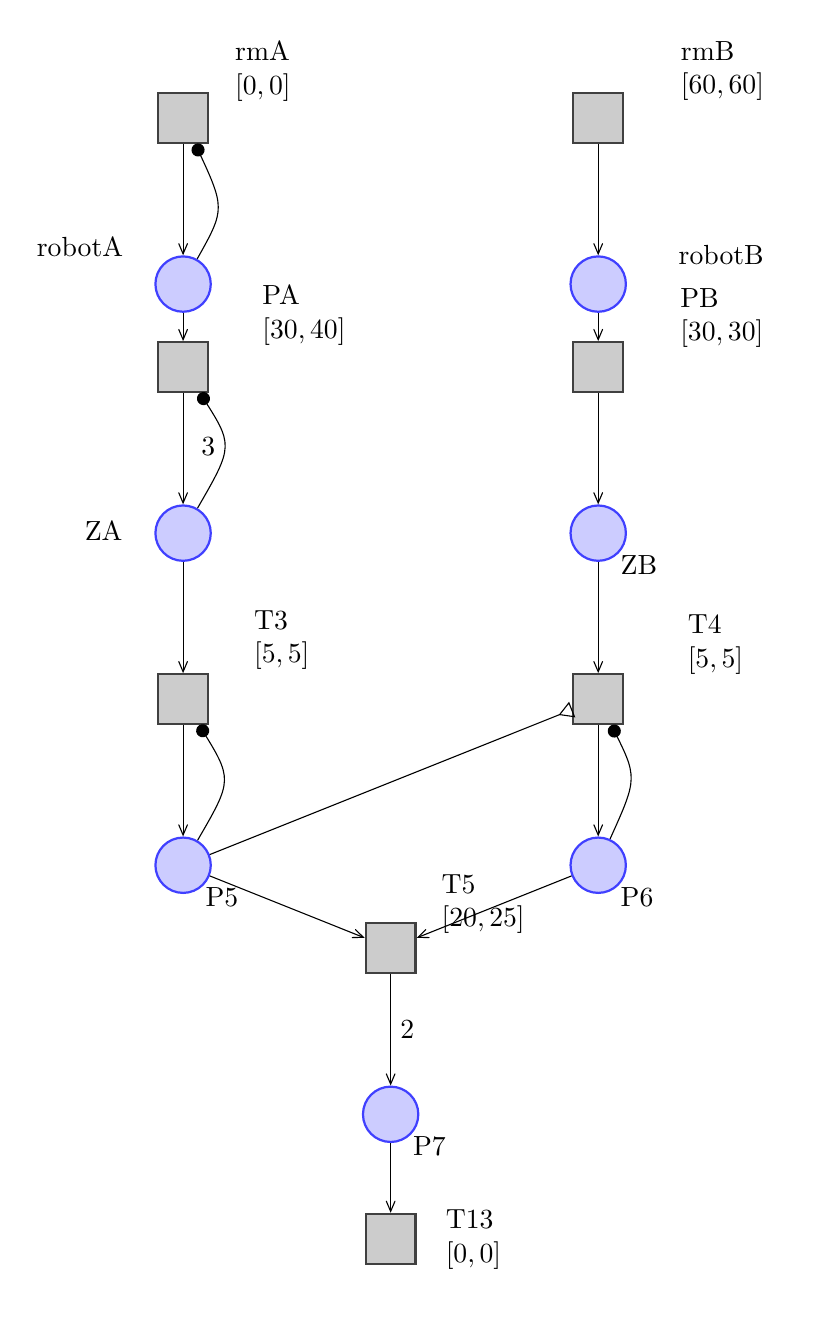
\begin{tikzpicture} 
	 [scale =1] 
	 \tikzset{node distance =2cm, bend angle=-45,auto}
	\tikzstyle{place}=[circle,thick,draw=blue!75,fill=blue!20,minimum size=20.0 pt]
	\tikzstyle{transition}=[rectangle,thick,draw=black!75,fill=black!20,minimum size=18.0 pt]
	\node [place,tokens=0](p1) at (226.0 pt,-181.0 pt)[label={[label distance=8.8pt]161.6:robotA}]{};
	\node [place,tokens=0](p2) at (226.0 pt,-271.0 pt)[label={[label distance=8.0pt]178.4:ZA}]{};
	\node [place,tokens=0](p3) at (376.0 pt,-181.0 pt)[label={[label distance=15.4pt]8.3:robotB}]{};
	\node [place,tokens=0](p4) at (376.0 pt,-271.0 pt)[label={[label distance=-3.9pt]-45.0:ZB}]{};
	\node [place,tokens=0](p5) at (226.0 pt,-391.0 pt)[label={[label distance=-3.9pt]-45.0:P5}]{};
	\node [place,tokens=0](p6) at (376.0 pt,-391.0 pt)[label={[label distance=-3.9pt]-45.0:P6}]{};
	\node [place,tokens=0](p7) at (301.0 pt,-481.0 pt)[label={[label distance=-3.9pt]-45.0:P7}]{};
	\node [transition] (t1)  at (226.0 pt,-211.0 pt)[label={[label distance=9.9pt]10.3:\begin{tabular}{l} PA \\  $ [30,40] $ \end{tabular}}]{};
	\node [transition] (t1)  at (226.0 pt,-211.0 pt)[label={[text=red,label distance=-15.7pt]45.0:\begin{tabular}{l} $  $ \\  \end{tabular}}]{};
	\node [transition] (t1)  at (226.0 pt,-211.0 pt)[label={[text=blue,label distance=-1.6pt]-26.6:\begin{tabular}{l} $  $ \\  \end{tabular}}]{};
	\draw[-angle 45] (p1) edge  (t1) ;
	\draw[-*] (p2) .. controls (244.3 pt,-239.3 pt) .. node { 3} (t1) ;
	\draw[-angle 45] (t1) edge  (p2) ;
	\node [transition] (t2)  at (376.0 pt,-211.0 pt)[label={[label distance=10.8pt]7.3:\begin{tabular}{l} PB \\  $ [30,30] $ \end{tabular}}]{};
	\node [transition] (t2)  at (376.0 pt,-211.0 pt)[label={[text=red,label distance=-15.7pt]45.0:\begin{tabular}{l} $  $ \\  \end{tabular}}]{};
	\node [transition] (t2)  at (376.0 pt,-211.0 pt)[label={[text=blue,label distance=-1.6pt]-26.6:\begin{tabular}{l} $  $ \\  \end{tabular}}]{};
	\draw[-angle 45] (p3) edge  (t2) ;
	\draw[-angle 45] (t2) edge  (p4) ;
	\node [transition] (t3)  at (226.0 pt,-331.0 pt)[label={[label distance=7.2pt]21.4:\begin{tabular}{l} T3 \\  $ [5,5] $ \end{tabular}}]{};
	\node [transition] (t3)  at (226.0 pt,-331.0 pt)[label={[text=red,label distance=-15.7pt]45.0:\begin{tabular}{l} $  $ \\  \end{tabular}}]{};
	\node [transition] (t3)  at (226.0 pt,-331.0 pt)[label={[text=blue,label distance=-1.6pt]-26.6:\begin{tabular}{l} $  $ \\  \end{tabular}}]{};
	\draw[-angle 45] (p2) edge  (t3) ;
	\draw[-*] (p5) .. controls (244.0 pt,-360.0 pt) ..  (t3) ;
	\draw[-angle 45] (t3) edge  (p5) ;
	\node [transition] (t4)  at (376.0 pt,-331.0 pt)[label={[label distance=13.7pt]11.0:\begin{tabular}{l} T4 \\  $ [5,5] $ \end{tabular}}]{};
	\node [transition] (t4)  at (376.0 pt,-331.0 pt)[label={[text=red,label distance=-15.7pt]45.0:\begin{tabular}{l} $  $ \\  \end{tabular}}]{};
	\node [transition] (t4)  at (376.0 pt,-331.0 pt)[label={[text=blue,label distance=-1.6pt]-26.6:\begin{tabular}{l} $  $ \\  \end{tabular}}]{};
	\draw[-angle 45] (p4) edge  (t4) ;
	\draw[-*] (p6) .. controls (390.3 pt,-359.3 pt) ..  (t4) ;
	\draw[-open triangle 60 reversed] (p5) edge  (t4) ;
	\draw[-angle 45] (t4) edge  (p6) ;
	\node [transition] (t5)  at (301.0 pt,-421.0 pt)[label={[label distance=-0.5pt]5.3:\begin{tabular}{l} T5 \\  $ [20,25] $ \end{tabular}}]{};
	\node [transition] (t5)  at (301.0 pt,-421.0 pt)[label={[text=red,label distance=-15.7pt]45.0:\begin{tabular}{l} $  $ \\  \end{tabular}}]{};
	\node [transition] (t5)  at (301.0 pt,-421.0 pt)[label={[text=blue,label distance=-1.6pt]-26.6:\begin{tabular}{l} $  $ \\  \end{tabular}}]{};
	\draw[-angle 45] (p5) edge  (t5) ;
	\draw[-angle 45] (p6) edge  (t5) ;
	\draw[-angle 45] (t5) edge node { 2} (p7) ;
	\node [transition] (t6)  at (376.0 pt,-121.0 pt)[label={[label distance=11.0pt]5.9:\begin{tabular}{l} rmB \\  $ [60,60] $ \end{tabular}}]{};
	\node [transition] (t6)  at (376.0 pt,-121.0 pt)[label={[text=red,label distance=-15.7pt]45.0:\begin{tabular}{l} $  $ \\  \end{tabular}}]{};
	\node [transition] (t6)  at (376.0 pt,-121.0 pt)[label={[text=blue,label distance=-1.6pt]-26.6:\begin{tabular}{l} $  $ \\  \end{tabular}}]{};
	\draw[-angle 45] (t6) edge  (p3) ;
	\node [transition] (t7)  at (226.0 pt,-121.0 pt)[label={[label distance=-0.1pt]9.2:\begin{tabular}{l} rmA \\  $ [0,0] $ \end{tabular}}]{};
	\node [transition] (t7)  at (226.0 pt,-121.0 pt)[label={[text=red,label distance=-15.7pt]45.0:\begin{tabular}{l} $  $ \\  \end{tabular}}]{};
	\node [transition] (t7)  at (226.0 pt,-121.0 pt)[label={[text=blue,label distance=-1.6pt]-26.6:\begin{tabular}{l} $  $ \\  \end{tabular}}]{};
	\draw[-*] (p1) .. controls (241.3 pt,-153.7 pt) ..  (t7) ;
	\draw[-angle 45] (t7) edge  (p1) ;
	\node [transition] (t8)  at (301.0 pt,-526.0 pt)[label={[label distance=1.0pt]0.0:\begin{tabular}{l} T13 \\  $ [0,0] $ \end{tabular}}]{};
	\node [transition] (t8)  at (301.0 pt,-526.0 pt)[label={[text=red,label distance=-15.7pt]45.0:\begin{tabular}{l} $  $ \\  \end{tabular}}]{};
	\node [transition] (t8)  at (301.0 pt,-526.0 pt)[label={[text=blue,label distance=-1.6pt]-26.6:\begin{tabular}{l} $  $ \\  \end{tabular}}]{};
	\draw[-angle 45] (p7) edge  (t8) ;
	\end{tikzpicture} 
	 \end{center} 
 } 
 \end{figure}

 
\end{document}
